% ==================================================
%	Dokumentklasse
% ==================================================

\documentclass[
	11pt,
	a4paper,
	fleqn,
	ngerman,
	parskip,
	toc=bibliography
]{scrartcl}

% input header

% ==================================================
%	Encoding
% ==================================================

\usepackage[utf8]{inputenc}
\usepackage[T1]{fontenc}
\usepackage{lmodern}
\usepackage{textcomp}

% ==================================================
%	Spracheinstellung
% ==================================================

\usepackage[ngerman]{babel}

% ==================================================
%	Referenzen
% ==================================================

\usepackage[ngerman]{varioref}
% Links im pdf
\usepackage[pdfborder={0 0 0}, hypertexnames=false]{hyperref}
% zusammen mit varioref, hyperref folgt damit
% z. B. in \vref{eq:1} -> in Gl. 1 auf Seite 4, cleveres referenzieren
\usepackage{cleveref}

% ==================================================
%	Grafiken, Abbildungen und Tabellen
% ==================================================

\usepackage{graphicx}
\usepackage{xcolor}
\usepackage[font=small, labelfont=bf, format=plain]{caption}
\usepackage{subcaption}
\usepackage{booktabs}
\usepackage[vflt]{floatflt}

\usepackage{rotating}

\usepackage{multicol}
\usepackage{multirow}

\usepackage{tikz}
\usetikzlibrary{shadows, calc, arrows, patterns}

\usepackage{tcolorbox}
\tcbuselibrary{skins, breakable, theorems}

\usepackage{pdfpages}

% ==================================================
%	Seiten-Layout und -Definitionen
% ==================================================

% Maße für DIN A4
\usepackage[a4paper]{geometry}

\clubpenalty=10000
\widowpenalty=10000
\displaywidowpenalty=10000

% Überschriften in Serifen
\setkomafont{sectioning}{\normalfont\normalcolor\bfseries}

% ==================================================
%	Float-Parameter
% ==================================================

% minimaler Anteil der Seite für den Text
\renewcommand{\textfraction}{0.05}
% maximaler Anteil der Seite für Floats am Anfang
\renewcommand{\topfraction}{0.95}
% maximaler Anteil der Seite für Floats am Enden
\renewcommand{\bottomfraction}{0.95}
% mininaler Anteil der Float-Seite für Text
\renewcommand{\floatpagefraction}{0.35}
% maximale Anzahl der Floats auf der Seite
\setcounter{totalnumber}{5}

% ==================================================
%	Fancy Header
% ==================================================

\usepackage{fancyhdr}
\pagestyle{fancy}

% Stil für gesamtes Dokument
\fancyhf{}

% Dicke der Linien ändern
\renewcommand{\headrulewidth}{1.0pt}
\renewcommand{\footrulewidth}{1.0pt}

% Abschnitte in Großschrift
\renewcommand{\sectionmark}[1]{\markright{\MakeUppercase{#1}}{}}
\renewcommand{\subsectionmark}[1]{}

% Die Positionen in Kopf- und Fußzeile füllen
\fancyhead[L]{%
	TU Dortmund
}
\fancyhead[R]{\tit}
\fancyfoot[L]{\rightmark}
\fancyfoot[R]{Seite \thepage}

\addtolength{\headheight}{2\baselineskip}

% Neudefinition von plain (wird auf Kapitel/Verzeichnis-Seiten verwendet)
\fancypagestyle{plain}{%
	\fancyhead[L]{}
	\fancyhead[R]{}
	\fancyfoot[L]{\rightmark}
	\fancyfoot[R]{Seite \thepage}
}

\fancypagestyle{firstpage}{%
	\fancyhf{}
	\fancyhead[L]{}
	\renewcommand{\footrulewidth}{0.0pt}
}

% ==================================================
%	Bibliograhphie
% ==================================================

\newcommand{\anhang}{%
	\clearpage
	\setcounter{page}{0}
	\pagenumbering{Roman}
	% Kapitelnummerierung in Großbuchstaben statt Zahlen
	\appendix
}

\newcommand{\referenzen}{
	% \renewcommand{\refname}{Quellenverzeichnis}
	\bibliographystyle{utphys}
	\bibliography{literatur}
}

% ========================================
%	Angaben für das Titelblatt
% ========================================

% einfaches Verändern des Titels/Versuchs in der Hauptdatei
\newcommand{\titel}[1]{\newcommand{\tit}{#1}}
\newcommand{\versuch}[1]{\newcommand{\ver}{Versuch #1}}

% ==================================================
%	Mathematik
% ==================================================

\usepackage{amsmath}
\usepackage{amsfonts}
\usepackage{amssymb}
\usepackage{amstext}
\usepackage{mathtools}
% für Einheitsmatrix '1'
\usepackage{bbm}

% Mathematik Font
% Palatino needs more leading (space between lines)
% \linespread{1.05}
% \usepackage[sc]{mathpazo}

\usepackage{fouriernc}
\usepackage{newcent}

% ==================================================
%	Physik
% ==================================================

\usepackage{upgreek}
\usepackage{physics}
\usepackage[nice]{units}
\usepackage[parse-numbers=false, per-mode=symbol]{siunitx}

% ==================================================
%	Sonstiges
% ==================================================

% rechnen mit LateX-Counter
\usepackage{calc}
% Euro-Zeichen
\usepackage{eurosym}
% für bessere Darstellung von Text (Abstände)
\usepackage{microtype}
% Einfügen von Text um Layout zu testen
\usepackage{lipsum}

\renewcommand{\i}{\text{i}}
\newcommand{\e}{\text{e}}


% ==================================================
%	Definitionen für das Dokument
% ==================================================


% ==================================================
%	Dokument beginnt
% ==================================================

\begin{document}

% ==================================================
%	Titelseite
% ==================================================

\titel{Tomographie}
\versuch{E14}
\newcommand{\thedate}{03.06.2015}

\begin{titlepage}

% Alles zentriert
\center

% ==================================================
%	Oberer Teil
% ==================================================

\textsc{\LARGE TU Dortmund}\\[1.5cm]
\textsc{\Large Fakultät Physik}\\[0.5cm]
\textsc{\large \ver}\\[0.5cm]

\rule{\textwidth}{1.6pt}\vspace*{-\baselineskip}\vspace*{2pt}
\rule{\textwidth}{0.4pt}\\[\baselineskip]

{ \huge \bfseries \tit}\\[0.2cm]

\rule{\textwidth}{0.4pt}\vspace*{-\baselineskip}\vspace{3.2pt}
\rule{\textwidth}{1.6pt}\\[\baselineskip]

% ==================================================
%	Authoren
% ==================================================

\begin{minipage}{0.4\textwidth}
\begin{flushleft} \large
Mario \textsc{Dunsch}\\
\small \href{mario.dunsch@tu-dortmund.de}{mario.dunsch@tu-dortmund.de}
\end{flushleft}
\end{minipage}
~
\begin{minipage}{0.4\textwidth}
\begin{flushright} \large
Dominik \textsc{Kahl}\\
\small \href{dominik.kahl@tu-dortmund.de}{dominik.kahl@tu-dortmund.de}
\end{flushright}
\end{minipage}\\[1cm]

% ==================================================
%	Datum
% ==================================================

{\large \thedate}\\[3cm]

\vfill

\end{titlepage}


% ==================================================
%	Inhaltsverzeichnis
% ==================================================

\thispagestyle{plain}
\tableofcontents
\newpage

% ==================================================
%	Hauptteil
% ==================================================

%
% ==================================================
%	Einleitung
% ==================================================

\section{Einleitung}
In dem Versuch V65 Röntgenreflektometrie wird mittels der Messung von 
Röntgenreflexen die Schichtdicke und Rauigkeit einer Probe bestimmt. In diesem 
Versuch wird dazu das D8-Labordiffraktometer von Bruker-AXS verwendet, um die 
Eigenschaften eines Polystyrol-Films , welcher auf einem Siliziumwafer 
aufgetragen wurde, zu bestimmen.
%
% ==================================================
%	Theorie
% ==================================================

\section{Theorie}
\subsection{Grundlagen der Röntgenbrechung an einer Grenzschicht}
Ein Röntgenstrahl, welcher durch den elektrischen Feldvektor $\vec{E}(\vec{r})=
\vec{E}_0 \e^{\i\vec{k}\vec{r}}$ beschrieben wird, wird beim Übergang vom Vakuum 
mit Brechungsindex $n_0=1$ in ein Medium mit Brechungsindex 
\begin{equation}
n=1-\delta+\i \beta \label{eq:Brechungsindex} 
\end{equation}
in Abhängigkeit vom Einfallswinkel $\alpha$ zu bestimmten Teilen reflektiert und 
transmittiert. Dabei beschreibt der Realteil des Brechungsindex die neue 
Wellenausbreitung, der Imaginärteil die Abschwächung der Amplitude im 
Medium. Die Schreibweise \eqref{eq:Brechungsindex} mit $\delta > 0$ 
impliziert bereits, dass $\mathfrak{Re}(n)<1$, d.h. die Lichtgeschwindigkeit im Medium ist 
größer als im Vakuum.
\begin{itemize}
\item[Aufgabe 1:] Das Medium wird als eine gleichmäßige Verteilung  
von $N$ harmonischen Oszillatoren der Eingenfrequenzen $\omega_j$ angenommen, sodass 
sich
\begin{equation}
n^2=1+N \frac{e^2}{\epsilon_0 \text{m}} \sum\limits_{j=1}^N \frac{f_j}
{\omega_j^2 - \omega^2-2\i\omega \eta_j}
\end{equation}
ergibt. dabei ist $\omega$ die Frequenz der einfallenden EM-Welle, m die 
Elektronenmasse, $e$ die Elementarladung, $\epsilon_0$ die 
Dielektrizitätskonstante, $\eta_j$ der Dämpfungsfaktor des $j$-ten Elektrons und 
$f_j$ die Stärke der angeregten Schwingung des $j$-ten Elektrons. Für 
Röntgenstrahlung gilt insbesondere $\omega < \omega_j$, sodass für homogene 
Medien die Näherungformel 
\begin{equation}
\delta=\frac{\lambda^2}{2 \uppi} r_e \rho
\end{equation}
für Röntgenstrahlung der Wellenlänge $\lambda$ und Elektronen mit Radius $r_e$ 
und Volumendichte $\rho$ gilt. Folglich ist $\delta$ für Röntgenstrahlung 
positiv und in einer Größenordnung von $10^{-6}$. 
\end{itemize}
Der Übergang in ein Medium mit kleinerem $\mathfrak{Re}(n)$ ermöglicht das Phänomen der 
Totalreflexion, sodass bei einem Einfallswinkel $\alpha_i < \alpha_\text{C}$ mit 
$\cos(\alpha_\text{C})=n$ kein Teil des Strahles transmittiert wird. Der 
Einfallswinkel $\alpha_i$ wir dabei zwischen Oberfläche und Wellenvektor gemessen. 
Näherungsweise ergibt sich $\alpha_\text{C}=\sqrt{2\delta}$.\\
Sind bei einer Röntgenreflexion $A$, $B$ und $C$ die Amplituden der 
einfallenden, der reflektierten und transmittierten Welle, so gilt für die 
Transmissions- und Reflexionskoeffizienten
\begin{align}
r&=r_s=\frac{B}{A}=\frac{k_\text{i,z}-k_\text{t,z}}{k_\text{i,z}-k_\text{t,z}} \label{eq:r} \\
t&=t_s=\frac{C}{A}= \frac{2 k_\text{i,z}}{k_\text{i,z}+k_\text{t,z}}
\end{align}
wobei $k_\text{i,z}=|\vec{k}|\sin(\alpha_i)$ und $k_\text{t,z}=|
\vec{k}|\sqrt{n^2-\cos^2(\alpha_i)}$ die $z$-Komponente des 
Wellenvektors 
$\vec{k}$ der einfallenden 
bzw. transmittierten Welle ist.
\begin{itemize}
\item[Aufgabe 2 a):] 
Für eine p-Polarisierte EM-Welle ergeben sich 
\begin{align}
r_p&= \frac{n^2 k_\text{i,z}-k_\text{t,z}}{n^2 k_\text{i,z}+k_\text{t,z}} \\
t_p&=\frac{2k_\text{i,z}}{n^2 k_\text{i,z}+k_\text{t,z}}
\end{align}
\item[Aufgabe 2 b):]
Da wie bereits gezeigt $\mathfrak{Re}(n)$ nur um $10^{-6}$ von $1$ abweicht, können in 
diesen Formeln die Faktoren $n$ vernachlässigt werden, sodass $r_s=r_p=r$ sowie 
$t_s=t_p=t$ gilt.
\end{itemize}
Die Fresnel-Reflektivität $R_\text{F}=r^2$ kann für Röntgenstrahlung für große 
Einfallswinkel $\alpha_\text{i}$ zu 
\begin{equation}
R_\text{F}\approx \left( \frac{\alpha_\text{C}}{2\alpha_\text{i}} \right)^4 \label{eq:Reflekt4}
\end{equation}
abgeschätzt werden. Dass heißt, die Intensität des Reflexes nimmt mit 
$\alpha_\text{i}^{-4}$ ab, sodass bei der Darstellung eine logarithmische Skala 
zu wählen ist.
\begin{itemize}
\item[Aufgabe 3:]
Zu zeigen ist, dass sich \eqref{eq:Reflekt4} aus \eqref{eq:r} ergibt.\\
Zunächst wird $r$ um $\frac{k_\text{i,z}+k_\text{t,z}}
{k_\text{i,z}+k_\text{t,z}}$ erweitert zu
\begin{align*}
r&=\frac{k_\text{i,z}^2-k_\text{t,z}^2}{(k_\text{i,z}+k_\text{t,z})^2}\\
\intertext{und $k_\text{i/t,z}$ eingesetzt,}
r&=\frac{|\vec{k}|^2\sin^2(\alpha_i)-|\vec{k}|^2 n^2+|\vec{k}|^2\cos^2 (\alpha_i)}
{\left(|\vec{k}|\sin(\alpha_i)+|\vec{k}|\sqrt{n^2-\cos^2(\alpha_i)}\right)^2} \quad 
.
\end{align*}
Nun wird die Bedingung $n=\cos(\alpha_\text{C})$ für den kritischen 
Winkel $\alpha_\text{C}$ der Totalreflexions eingesetzt, und eine 
Taylorentwicklung 2.Ordnung von $\sin$ und $\cos$ für kleine Winkel $\alpha_i$ vorgenommen
\begin{align*}
r&=\frac{1-\cos^2(\alpha_\text{C})}{\left( \sin(\alpha_i)+\sqrt{\cos^2(\alpha_\text{C})-\cos^2(\alpha_i)} \right)^2} \\
&\approx \frac{\alpha^2_\text{C}}{\left( \alpha_i+\sqrt{\alpha_i^2-\alpha_\text{C}^2} \right)^2}
\end{align*}
Nun soll das Verhalten der Fresnel-Reflektivität für große 
Einfallswinkel $\alpha_i >> \alpha_\text{C} $ betrachtet werden, 
sodass $\alpha_i+\alpha_\text{C}\approx \alpha_\text{i}$ genähert 
werden kann.
\begin{equation}
r\approx \frac{\alpha_\text{C}}{(2\alpha_i)^2}
\end{equation}
und damit
\begin{equation}
R_\text{F}=r^2\approx \left(\frac{\alpha_\text{C}}{2\alpha_i} 
\right)^4 \quad .
\end{equation}
\end{itemize}
\subsection{Mehrschichtsysteme}
Nun soll das Problem der Röntgenreflexion auf ein System mit mehreren 
Grenzschichten erweitert werden, speziell wird der im Experiment vorliegende 
Fall einer Probenschicht auf einem Trägermaterial thematisiert.\\
Der Röntgenstrahl fällt aus dem Medium 1 mit $n_1=1$ auf das Medium 
2 (Brechungsindex $n_2$, Schichtdicke $d$) und wird an der Grenzschicht zu $r_2$ 
reflektiert und zu $t_2$ 
transmittiert. Der transmittierte Teilstrahl durchdringt das Medium 2 und trifft 
auf das Trägermaterial (Brechungsindex $n_3$, Schichtdicke $\to \infty$) und wird 
dort wiederum zu $r_3$ reflektiert und zu $t_3$ transmittiert. Nach Austritt der 
reflektierten Strahlen ergibt sich durch deren Überlagerung eine 
Gesamtreflektivität $R$, welche aufgrund von Interferenzen zwischen den 
reflektierten Strahlen für steigende Einfallswinkel $\alpha$ oszilliert. Sind 
$\alpha_1$ und $\alpha_2$ zwei benachbarte Extremstellen dieser Oszillation, so 
lässt sich die Schichtdicke über
\begin{equation}
d \approx \frac{\lambda}{2(\alpha_2 -\alpha_1)}
\end{equation}
abschätzen.
\begin{itemize}
\item[Aufgabe 4:]
Der Gangunterschied $\Delta l_n$ zwischen zwei Minima muss $\Delta l_n=
(2n+1)/2 \lambda$ betragen, damit die Phasendifferenz $\uppi$ ist. Außerdem 
gilt wegen der Geometrie des Problems, dass $\Delta l_n = 2 d/\sin(\alpha_n)$. 
Aus der Berechnung von $\Delta l_{n+1}- \Delta l_n$ mit $\sin(\alpha)\approx 
\alpha$ (Kleinwinkelnäherung) folgt die angegebene Gleichung für die 
Schichtdicke $d$. Dies ist in Abbildung \ref{fig:Bild} veranschaulicht.
\begin{figure}[h]
\centering
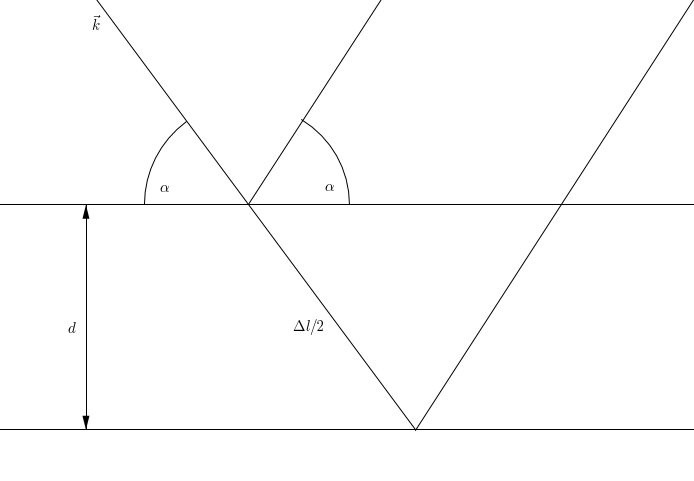
\includegraphics[scale=0.4]{../skript/Bild.png}
\caption{Veranschaulichung der geometrischen Bedingungen zwischen der 
Schichtdicke $d$, dem Einfallswinkel $\alpha$ und dem Gangunterschied $\Delta 
l$.}
\label{fig:Bild}
\end{figure}
\end{itemize}
Die Amplituden $R_j$ und $T_j$ der reflektierten und transmittierten Welle der 
$j$-ten Grenzschicht stehen im Verhältnis
\begin{equation}
X_j:=\frac{R_j}{T_j}=\e^{-2\i k_\text{z,j}z_j} \frac{r_{j,j+1}+X_{j+1}\e^{2\i 
k_\text{z,j+1}z_j}}{1+r_{j,j+1}X_{j+1}\e^{2\i k_{z,j+1}z_j}}
\end{equation}
mit $r_{j,j+1}=\frac{k_{z,j}-k_{z,j+1}}{k_{z,j}+k_{z,j+1}}$ und $k_{z,j}=|
\vec{k}|\sqrt{n_j^2-\cos^2 \alpha_i}$.
\begin{itemize}
\item[Aufgabe 5:]
Eine Darstellung der Gesamtreflektivität $X$ in Abhängigkeit vom Einfallswinkel 
$\alpha$ ist in Abbildung \ref{fig:Mehrschicht} zu sehen.
\begin{figure}[h]
\centering
\includegraphics[scale=1]{../skript/reflektivitaet.pdf}
\caption{Darstellung von $X$ in Abhängigkeit vom Einfallswinkel $\alpha$ für 
eine Rauigkeit von $\sigma=6\AA$ und $n_\text{Substrat}=1-1\times 10^{-6}$.}
\label{fig:Mehrschicht}
\end{figure}
\end{itemize}


\subsection{Die Rauigkeit einer Grenzschicht}
Bisher wurde stets die Annahme gemacht, dass die Grenzschichten eben und ohne 
weitere Struktur sind. Nun wird die Rauigkeit der $j$-ten Genzschicht (bei 
$z=z_j)$ durch eine 
Wahrscheinlichkeitsdichte $P_j$ modelliert, sodass $P_j(z)\,\text{d}z$ die 
Wahscheinlichkeit ist, dass die Grenzschicht in $\text{d}z$ um $z$ liegt. Als 
Maß für die Rauigkeit wird dann
\begin{equation}
\sigma_j^2=\int (z-z_j)^2 P_j(z)\, \text{d}z
\end{equation}
gewählt. Als modifizierter Brechungsindex wird
\begin{equation}
n(z)=\frac{n_j+n_{j+1}}{2}- \frac{n_j-n_{j+1}}{2} \text{erf}\left(\frac{z-z_j}
{\sqrt{2 \sigma^2_j}}  \right)
\end{equation}
benutzt, sodass sich $P_j(z)$ als Gaußfunktion ergibt. Es folgen die neuen 
Fresnel-Koeffizienten
\begin{align}
\tilde{r}_{j,j+1}&=r_{j,j+1} \e^{-2 k_\text{z,j}k_\text{z,j+1}\sigma_j^2} \\
\tilde{t}_{j,j+1}&=t_{j,j+1} \e^{(k_\text{z,k}-k_\text{z,j+1})^2 \sigma_j^2/2}
\end{align}
\begin{itemize}
\item[Aufgabe 6:]
Eine Darstellung des Gesamtreflektivität für ein System mit einer nicht 
verschwindenden Rauigkeit ist in Abbildung \ref{fig:Rauigkeit} zu sehen.
\begin{figure}[h]
\centering
\includegraphics[scale=1]{../skript/reflektivitaet_rau.pdf}
\caption{Darstellung von $X$ in Abhängigkeit vom Einfallswinkel $\alpha$ für 
eine Rauigkeit von $\sigma=6\AA$ und $n_\text{Substrat}=1-1\times 10^{-6}$.}
\label{fig:Rauigkeit}
\end{figure}
\end{itemize}



%\cite{FP}
% ==================================================
%	Aufbau
% ==================================================

\section{Aufbau}
\begin{figure}
\centering 
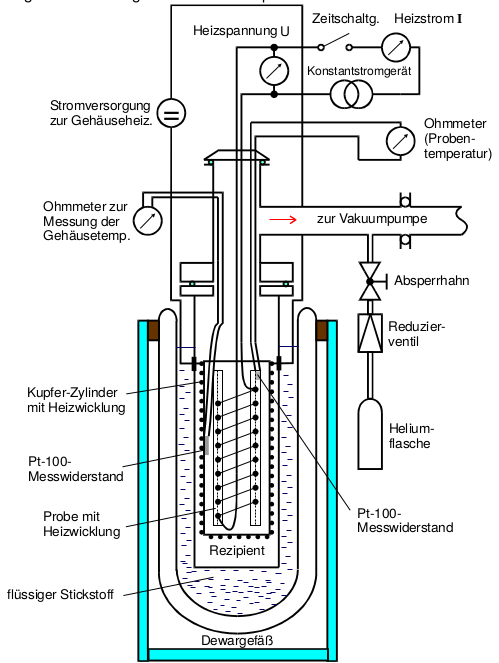
\includegraphics[scale=1]{figures/setup.pdf}
\caption{Schematische Abbildung des Versuchsaufbaus. \cite{FP}}
\label{fig:aufbau:setup}
\end{figure}
Der Versuchsaufbau ist in Abbildung \ref{fig:aufbau:setup} zu sehen. Der 
Rezipient befindet sich in einem Gehäuse, das mittels einer Vakuumpumpe 
evakuiert werden kann. Über ein Ventil kann das Gehäuse mit Helium befüllt 
werden. Rezipient und Gehäuse besitzen jeweils eine eigene Heizwicklung, sodass 
diese über getrennte Stromversorgungen einzeln geheizt werden können. Die 
Temperaturmessung geschieht mittels Widerstandsmessung eines Pt-100-Messwiderstandes, 
für den die Beziehung 
\begin{equation}
T = 0.00135 R^2 + 2.296 R -243.02
\end{equation}
zwischen dem gemessenen Widerstandswert $R$ in $\Omega$ und der Temperatur $T$ in 
$\si{\celsius}$ gilt. Das Gehäuse befindet sich in einem Dewargefäß.

% ==================================================
%	Durchführung
% ==================================================

\section{Durchführung}

\subsection{Einfaches Spektrometer}
\label{sub:einfaches_spektrometer}

\subsubsection{Eigenrauschen des Rauschspektrometers}
\label{ssub:eigenrauschen_des_rauschspektrometers}

Zur Bestimmung des Eigenrauschens des einfachen Rauschspektrometers wird die
Verstärkerschaltung aus Abbildung~\ref{fig:spektrometer} verwandt, wobei der
Widerstand durch einen Kurzschluss ersetzt wird.
Der Bandpass wird dabei so eingestellt, dass nur Frequenzen zwischen
\SI{20}{\kilo\hertz}und \SI{30}{\kilo\hertz} durchgelassen
werden.  Die Ausgangsspannung besteht nun lediglich aus dem Rauschen der
Verstärkerschaltung, das bei allen anderen Messungen den Untergrund darstellt.

\subsubsection{Durchlasskurve des Bandfilters}
\label{ssub:durchlasskurve_des_bandfilters}

Die Durchlasskurve des Bandfilters wird mit dem Aufbau aus
Abbildung~\ref{fig:spektrometer} vermessen.
Hierbei wird anstelle des Widerstands ein Frequenzgenerator angeschlossen.
Der Bandpass wird hierbei aus der vorigen Messung nicht verstellt.
Die Frequenzen werden nun logarithmisch über drei Zehnerpotenzen variiert.
Die Ausgangsspannungen und die Verstärkungen des Nachverstärkers werden notiert.

\subsubsection{Rauschmessung des Widerstands}
\label{ssub:rauschmessung_des_widerstands}

Es wird nun die Ausgangsspannung in Abhängigkeit des Widerstandes gemessen und
die jeweilige Nachverstärkung notiert.
Hierzu werden zwei Potentiometer verwandt mit den Bereichen
\SIrange[range-phrase=--, range-units=single]{0}{1000}{\ohm}
und
\SIrange[range-phrase=--, range-units=single]{1}{10}{\kilo\ohm}.

\subsection{Korrelatorschaltung}
\label{sub:korrelatorschaltung}

\subsubsection{Eigenrauschen des Spektrometers}
\label{ssub:eigenrauschen_des_spektrometers}

Auch bei der Korrelatorschaltung wird zunächst das Eigenrauschen der 
Verstärkerschaltung gemessen.

\subsubsection{Durchlasskurve des Selektivverstärkers}
\label{ssub:durchlasskurve_des_selektivverstärkers}

Zur Bestimmung der Durchlasskurve des Selektivverstärkers wird die Schaltung
aus Abbildung~\ref{fig:korrelator} verwandt, wobei anstelle des Widerstands
wieder ein Frequenzgenerator angeschlossen wird.
Anschließend wird die Ausgangsspannung zu Frequenzen zwischen
\SIrange{3}{60}{\kilo\hertz} vermessen.

\subsubsection{Rauschmessung des Widerstands mit der Korrelatorschaltung}
\label{ssub:rauschmessung_des_widerstands_mit_der_korrelatorschaltung}

Die Rauschmessung erfolgt analog zu
Abschnitt~\ref{ssub:rauschmessung_des_widerstands}, wobei jedoch
Schaltung~\ref{fig:korrelator} verwandt wird.

\subsection{Vermessung der Hochvakuumdiode mit Reinmetallkathode}
\label{sub:vermessung_der_hochvakuumdiode_mit_reinmetallkathode}

\subsubsection{Kennlinie der Diode}
\label{ssub:kennlinie_der_diode}

Zur Vermessung der Kennlinie wird die Schaltung aus Abbildung~\ref{fig:schrot}
verwandt. Hierbei wird nun die Heizspannung varriert und anschließend die
Ausgangsspannung in Abhängigkeit der Anodenspannung gemessen.

\subsubsection{Messung zur Bestimmung der Elementarladung}
\label{ssub:messung_zur_bestimmung_der_elementarladung}

Hierbei wird die Anodenstrom auf \SI{130}{\volt} eingestellt und die
Ausgangsspannung in Abhängigkeit des Anodenstroms gemessen.
Für diese Messung wird der Bandpassfilter mit $\Delta\nu = \SI{20}{\kilo\hertz}$
in dem Bereich \SIrange{100}{120}{\kilo\hertz} benutzt. Zudem werden die
Nachverstärkungen notiert.

\subsubsection{Messung des Frequenzspektrums}
\label{ssub:messung_des_frequenzspektrums}

Das Frequenzspektrum wird bei einem konstanten Heizstrom von \SI{0.8}{\ampere}
einer Anodenspannung von \SI{130}{\volt} und einem Anodenstrom von
\SI{1}{\milli\ampere} aufgenommen. Hierbei arbeitet die Diode im
Sättigungsbetrieb.
Der Innenwiderstand der Diode beträgt hier \SI{4680}{\ohm}.
Bei der Messung werden die Frequenzen über vier Zehnerpotenzen
\SIrange{0.010}{460}{\kilo\hertz} variiert. Bei Frequenzen von
\SIrange{100}{460}{\kilo\hertz} wird ein Bandpassfilter verwandt und sonst der
Selektivverstärker. Es werden die Ausgangsspannungen und die Nachverstärkungen
notiert.

\subsection{Vermessung der Hochvakuumdiode mit Oxydkathode}
\label{sub:vermessung_der_hochvakuumdiode_mit_oxydkathode}

Die Messung wird hier analog zu der in
Abschnitt~\ref{ssub:messung_des_frequenzspektrums} durchgeführt.
Der Innenwiderstand beträgt hier \SI{2200}{\ohm}.


% ==================================================
%	Definitionen
% ==================================================

\newcommand{\CU}{RG-58C/U}
\newcommand{\BU}{RG-58B/U}

% ==================================================
%	Auswertung
% ==================================================

\section{Auswertung}

%%%%%%%%%%%%%%%%%%%%%%%%%%%%%%%%%%%%%%%%%%%%%%%%%%%%%%%%%%%%%%%%%%%%%%%%%%%
%                           Leitungskonstanten                            %
%%%%%%%%%%%%%%%%%%%%%%%%%%%%%%%%%%%%%%%%%%%%%%%%%%%%%%%%%%%%%%%%%%%%%%%%%%%

\subsection{Leitungskonstanten}
\label{sub:leitungskonstanten}

Es sollen die mit einem LCU-Messgerät bestimmen Leitungskonstanten
$R$, $L$ und $C$ in Abhängigkeit der Frequenz $\nu$ von drei Koaxialkabel,
einem langen und einem kurzen \CU\ sowie einem kurzen \BU\ dargestellt werden.
Des weiteren soll der Leitwert $G$ berechnet und ebenfalls graphisch
dargestellt werden.
Die im Versuch gemessenen Werte befinden sich dabei in den
Tabellen~\ref{tab:Leitungskonstanten_50k},~\ref{tab:Leitungskonstanten_50l}
und~\ref{tab:Leitungskonstanten_75k}.
Die in den Tabellen angegebenen Daten sind in den Abbildungen~\ref{fig:R_50k}
bis~\ref{fig:G_75k} graphisch dargestellt.

% ==================================================
% 	Tabellen
% ==================================================

\begin{table}[htpb]
  \centering
  \begin{tabular}{ccccc}
    \midrule
    \midrule
    $\nu / \si{kHz}$        & $C / \si{\pico\farad}$     & $R / \si{\ohm}$ &
    $L / \si{\micro\henry}$ & $G / \si{\milli\siemens}$ \\
    \midrule
    \phantom{0}0.2    & 990.14            & 0.5228            & 2.50              & 207.1            \\
\phantom{0}0.4    & 990.07            & 0.5220            & 3.10              & 166.7            \\
\phantom{0}0.6    & 990.10            & 0.5217            & 3.10              & 166.6            \\
\phantom{0}0.8    & 990.14            & 0.5215            & 3.20              & 161.4            \\
\phantom{0}1.0    & 990.04            & 0.5213            & 3.20              & 161.3            \\
\phantom{0}2.0    & 989.90            & 0.5212            & 3.18              & 162.2            \\
\phantom{0}3.0    & 989.93            & 0.5210            & 3.18              & 162.2            \\
\phantom{0}4.0    & 989.88            & 0.5210            & 3.19              & 161.7            \\
\phantom{0}5.0    & 989.90            & 0.5211            & 3.18              & 162.2            \\
\phantom{0}6.0    & 989.91            & 0.5211            & 3.18              & 162.2            \\
\phantom{0}7.0    & 989.93            & 0.5212            & 3.18              & 162.2            \\
\phantom{0}8.0    & 989.94            & 0.5213            & 3.18              & 162.3            \\
\phantom{0}9.0    & 989.92            & 0.5215            & 3.18              & 162.3            \\
10.0              & 989.95            & 0.5216            & 3.18              & 162.4            \\
11.0              & 990.01            & 0.5218            & 3.18              & 162.4            \\
12.0              & 990.05            & 0.5219            & 3.18              & 162.5            \\
13.0              & 990.07            & 0.5223            & 3.18              & 162.6            \\
14.0              & 990.12            & 0.5225            & 3.18              & 162.7            \\
15.0              & 990.13            & 0.5220            & 3.18              & 162.5            \\
16.0              & 990.01            & 0.5216            & 3.18              & 162.4            \\
17.0              & 990.01            & 0.5215            & 3.18              & 162.4            \\
18.0              & 990.04            & 0.5219            & 3.18              & 162.5            \\
19.0              & 989.98            & 0.5222            & 3.18              & 162.6            \\
20.0              & 989.96            & 0.5226            & 3.18              & 162.7            \\
    \midrule
    \midrule
  \end{tabular}
  \caption{Darstellung der in Abhängigkeit der Frequenz $\nu$ gemessenen
      Leitungskonstanten $R$, $L$ und $C$ für das kurze \CU-Kabel.}
\label{tab:Leitungskonstanten_50k}
\end{table}

\begin{table}[htpb]
  \centering
  \begin{tabular}{ccccc}
    \midrule
    \midrule
    $\nu / \si{kHz}$        & $C / \si{\nano\farad}$     & $R / \si{\ohm}$ &
    $L / \si{\micro\henry}$ & $G / \si{\siemens}$ \\
    \midrule
    \phantom{0}0.2    & 8.5013            & 4.1958            & 24.9              & 1.4              \\
\phantom{0}0.4    & 8.5015            & 4.1992            & 26.4              & 1.4              \\
\phantom{0}0.6    & 8.5016            & 4.1989            & 26.2              & 1.4              \\
\phantom{0}0.8    & 8.5014            & 4.1988            & 27.0              & 1.3              \\
\phantom{0}1.0    & 8.5012            & 4.1988            & 26.0              & 1.4              \\
\phantom{0}2.0    & 8.5004            & 4.1991            & 26.0              & 1.4              \\
\phantom{0}3.0    & 8.5003            & 4.1979            & 25.9              & 1.4              \\
\phantom{0}4.0    & 8.5003            & 4.2010            & 25.9              & 1.4              \\
\phantom{0}5.0    & 8.5003            & 4.2014            & 25.9              & 1.4              \\
\phantom{0}6.0    & 8.5007            & 4.2022            & 25.9              & 1.4              \\
\phantom{0}7.0    & 8.5011            & 4.2058            & 25.9              & 1.4              \\
\phantom{0}8.0    & 8.5012            & 4.2062            & 25.9              & 1.4              \\
\phantom{0}9.0    & 8.5018            & 4.2094            & 25.9              & 1.4              \\
10.0              & 8.5022            & 4.2093            & 25.9              & 1.4              \\
11.0              & 8.5028            & 4.2114            & 25.9              & 1.4              \\
12.0              & 8.5034            & 4.2135            & 25.9              & 1.4              \\
13.0              & 8.5040            & 4.2177            & 25.9              & 1.4              \\
14.0              & 8.5048            & 4.2191            & 25.9              & 1.4              \\
15.0              & 8.5056            & 4.2202            & 25.9              & 1.4              \\
16.0              & 8.5064            & 4.2235            & 25.9              & 1.4              \\
17.0              & 8.5071            & 4.2266            & 25.9              & 1.4              \\
18.0              & 8.5079            & 4.2297            & 25.9              & 1.4              \\
19.0              & 8.5075            & 4.2345            & 25.9              & 1.4              \\
20.0              & 8.5082            & 4.2690            & 25.9              & 1.4              \\
    \midrule
    \midrule
  \end{tabular}
  \caption{Darstellung der in Abhängigkeit der Frequenz $\nu$ gemessenen
      Leitungskonstanten $R$, $L$ und $C$ für das lange \CU-Kabel.}
\label{tab:Leitungskonstanten_50l}
\end{table}

\begin{table}[htpb]
  \centering
  \begin{tabular}{ccccc}
    \midrule
    \midrule
    $\nu / \si{kHz}$        & $C / \si{\pico\farad}$     & $R / \si{\ohm}$ &
    $L / \si{\micro\henry}$ & $G / \si{\milli\siemens}$ \\
    \midrule
    \phantom{0}0.20   & 674.3300          & 1.9534            & 5.0               & 263.4            \\
\phantom{0}0.40   & 674.4100          & 1.9521            & 6.2               & 212.3            \\
\phantom{0}0.60   & 674.4700          & 1.9517            & 6.1               & 215.8            \\
\phantom{0}0.80   & 674.4600          & 1.9515            & 6.1               & 215.8            \\
\phantom{0}1.00   & 674.4400          & 1.9512            & 6.1               & 215.7            \\
\phantom{0}2.00   & 674.2300          & 1.9526            & 6.1               & 216.2            \\
\phantom{0}3.00   & 674.1900          & 1.9554            & 6.0               & 217.9            \\
\phantom{0}4.00   & 674.1900          & 1.9590            & 6.0               & 219.8            \\
\phantom{0}5.00   & 674.2000          & 1.9636            & 6.0               & 221.8            \\
\phantom{0}6.00   & 674.2200          & 1.9690            & 5.9               & 224.2            \\
\phantom{0}7.00   & 674.2300          & 1.9755            & 5.9               & 226.1            \\
\phantom{0}8.00   & 674.1800          & 1.9822            & 5.8               & 230.0            \\
\phantom{0}9.00   & 674.2000          & 1.9895            & 5.8               & 233.3            \\
10.00             & 674.1700          & 1.9971            & 5.7               & 236.6            \\
11.00             & 674.1900          & 2.0048            & 5.6               & 240.1            \\
12.00             & 674.2100          & 2.0127            & 5.6               & 243.6            \\
13.00             & 674.2500          & 2.0205            & 5.5               & 247.7            \\
14.00             & 674.2600          & 2.0281            & 5.4               & 251.4            \\
15.00             & 674.2700          & 2.0354            & 5.4               & 255.1            \\
16.00             & 674.2600          & 2.0428            & 5.3               & 258.4            \\
17.00             & 674.2600          & 2.0500            & 5.3               & 262.3            \\
18.00             & 674.3500          & 2.0570            & 5.2               & 266.2            \\
19.00             & 674.4000          & 2.0636            & 5.2               & 269.7            \\
20.00             & 674.3800          & 2.0699            & 5.1               & 273.2            \\
    \midrule
    \midrule
  \end{tabular}
  \caption{Darstellung der in Abhängigkeit der Frequenz $\nu$ gemessenen
      Leitungskonstanten $R$, $L$ und $C$ für das \BU-Kabel.}
\label{tab:Leitungskonstanten_75k}
\end{table}

% ==================================================
% 	Plots
% ==================================================

\begin{figure}[t]
	\centering
	\includegraphics[scale=1.0]{bilder/R_50k.pdf}
	\caption{Darstellung des Widerstandes $R$ in Abhängigkeit der Frequenz $\nu$
	für das kurze \CU-Kabel.}
	\label{fig:R_50k}
	\includegraphics[scale=1.0]{bilder/R_50l.pdf}
	\caption{Darstellung des Widerstandes $R$ in Abhängigkeit der Frequenz $\nu$
	für das lange \CU-Kabel.}
	\label{fig:R_50l}
\end{figure}

\begin{figure}[h!]
	\centering
	\includegraphics[scale=1.0]{bilder/R_75k.pdf}
	\caption{Darstellung des Widerstandes $R$ in Abhängigkeit der Frequenz $\nu$
	für das \BU-Kabel.}
	\label{fig:R_75k}
	\includegraphics[scale=1.0]{bilder/C_50k.pdf}
	\caption{Darstellung der Kapazität $C$ in Abhängigkeit der Frequenz $\nu$
	für das kurze \CU-Kabel.}
	\label{fig:C_50k}
\end{figure}

\begin{figure}[h!]
	\centering
	\includegraphics[scale=1.0]{bilder/C_50l.pdf}
	\caption{Darstellung der Kapazität $C$ in Abhängigkeit der Frequenz $\nu$
	für das lange \CU-Kabel.}
	\label{fig:C_50l}
	\includegraphics[scale=1.0]{bilder/C_75k.pdf}
	\caption{Darstellung der Kapazität $C$ in Abhängigkeit der Frequenz $\nu$
	für das \BU-Kabel.}
	\label{fig:C_75k}
\end{figure}

\begin{figure}[h!]
	\centering
	\includegraphics[scale=1.0]{bilder/L_50k.pdf}
	\caption{Darstellung der Induktivität $L$ in Abhängigkeit der Frequenz $\nu$
	für das kurze \CU-Kabel.}
	\label{fig:L_50k}
	\includegraphics[scale=1.0]{bilder/L_50l.pdf}
	\caption{Darstellung der Induktivität $L$ in Abhängigkeit der Frequenz $\nu$
	für das lange \CU-Kabel.}
	\label{fig:L_50l}
\end{figure}

\begin{figure}[h!]
	\centering
	\includegraphics[scale=1.0]{bilder/L_75k.pdf}
	\caption{Darstellung der Induktivität $L$ in Abhängigkeit der Frequenz $\nu$
	für das \BU-Kabel.}
	\label{fig:L_75k}
	\includegraphics[scale=1.0]{bilder/G_50k.pdf}
	\caption{Darstellung des Leitwerts $G$ in Abhängigkeit der Frequenz $\nu$
	für das kurze \CU-Kabel.}
	\label{fig:G_50k}
\end{figure}

\begin{figure}[h!]
	\centering
	\includegraphics[scale=1.0]{bilder/G_50l.pdf}
	\caption{Darstellung des Leitwerts $G$ in Abhängigkeit der Frequenz $\nu$
	für das lange \CU-Kabel.}
	\label{fig:G_50l}
	\includegraphics[scale=1.0]{bilder/G_75k.pdf}
	\caption{Darstellung des Leitwerts $G$ in Abhängigkeit der Frequenz $\nu$
	für das \BU-Kabel.}
	\label{fig:G_75k}
\end{figure}

%%%%%%%%%%%%%%%%%%%%%%%%%%%%%%%%%%%%%%%%%%%%%%%%%%%%%%%%%%%%%%%%%%%%%%%%%%%
%                           Dämpfungskonstante                            %
%%%%%%%%%%%%%%%%%%%%%%%%%%%%%%%%%%%%%%%%%%%%%%%%%%%%%%%%%%%%%%%%%%%%%%%%%%%

\clearpage
\subsection{Dämpfungskonstante}
\label{sub:d_mpfungskonstante}

Es soll die Frequenzabhängigkeit der Dämpfungskonstante des langen
\CU-Kabels bestimmt werden. %TODO
Dazu wird ein Signal auf das kurze \CU-Kabel gegeben und die Dämpfung $L_0$
der ersten Oberwelle bestimmt.
Anschließend wird das Signal auf das zu analysierende lange
\CU-Kabel gegeben und ebenfalls wieder die Dämpfung $L_1$ der ersten Oberwelle
bestimmt.
Die Dämpfung wird dabei in \si{dBm} gemessen. Der Pegel ist damit durch
\begin{equation}
	L = 10 \log(\frac{P}{1\si{\milli\watt}})
\end{equation}
gegeben. Daher kann die Dämpfung in \si{\dB} des \CU-Kabel durch
\begin{equation}
	A = L_1 - L_0
\end{equation}
bestimmt werden. In Tabelle \ref{tab:Attenuation} sind die gemessenen Pegel und
die berechnete Dämpfung angegeben. Die berechneten Werte sind in
\ref{fig:bilder/alpha} graphisch dargestellt.

\begin{table}[hb]
  \centering
  \begin{tabular}{ccc|c}
    \midrule
    \midrule
    $\nu / \si{\kHz}$ & $L_0 / \si{dBm}$ & $L_1 / \si{dBm}$ &
    $A / \si{\dB}$ \\
    \midrule
    \phantom{0}2\phantom{.} & --8.3             & \phantom{0}--8.9  & --0.6            \\
\phantom{0}4\phantom{.} & --6.1             & \phantom{0}--7.8  & --1.7            \\
\phantom{0}6\phantom{.} & --5.4             & \phantom{0}--7.9  & --2.5            \\
\phantom{0}8\phantom{.} & --4.5             & \phantom{0}--7.5  & --3.0            \\
10\phantom{.}     & --4.6             & \phantom{0}--8.0  & --3.4            \\
12\phantom{.}     & --4.9             & \phantom{0}--8.5  & --3.6            \\
14\phantom{.}     & --4.5             & \phantom{0}--8.8  & --4.3            \\
16\phantom{.}     & --5.7             & \phantom{0}--9.9  & --4.2            \\
18\phantom{.}     & --5.5             & --10.1            & --4.6            \\
20\phantom{.}     & --5.7             & --10.6            & --4.9            \\
22\phantom{.}     & --5.8             & --11.0            & --5.2            \\
24\phantom{.}     & --5.5             & --11.2            & --5.7            \\
26\phantom{.}     & --5.7             & --11.6            & --5.9            \\
28\phantom{.}     & --5.9             & --12.0            & --6.1            \\
30\phantom{.}     & --5.9             & --12.2            & --6.3            \\
32\phantom{.}     & --5.7             & --12.3            & --6.6            \\
34\phantom{.}     & --6.0             & --12.9            & --6.9            \\
36\phantom{.}     & --6.0             & --13.2            & --7.2            \\
38\phantom{.}     & --5.9             & --13.4            & --7.5            \\
40\phantom{.}     & --6.0             & --13.8            & --7.8            \\
42\phantom{.}     & --6.0             & --14.1            & --8.1            \\
44\phantom{.}     & --6.1             & --14.4            & --8.3            \\
46\phantom{.}     & --4.9             & --13.8            & --8.9            \\
48\phantom{.}     & --5.4             & --14.5            & --9.1            \\
50\phantom{.}     & --5.2             & --14.3            & --9.1            \\
    \midrule
    \midrule
  \end{tabular}
  \caption{Gemessene Werte der Dämpfung des kurzen \CU-Kabels $A_0$ und
  des langen \CU-Kabels im Bezug zu \SI{1}{\milli\watt}
  sowie die berechnete Dämpfung A des \CU-Kabels.}
  \label{tab:Attenuation}
\end{table}

\begin{figure}[ht]
	\centering
	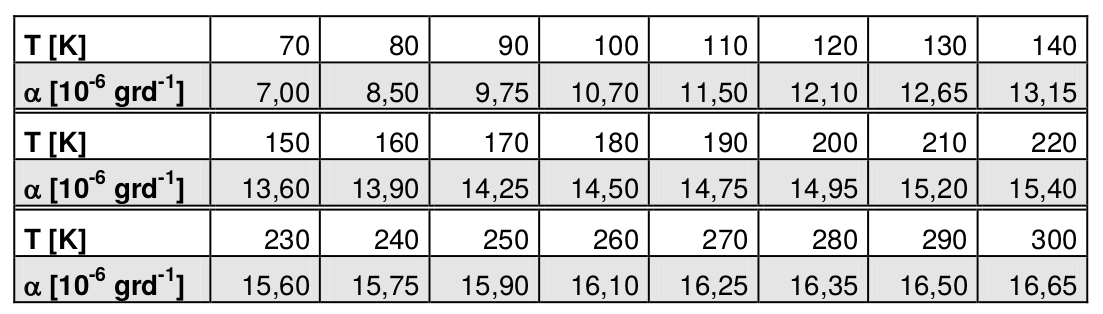
\includegraphics[scale=1.0]{bilder/alpha.pdf}
	\caption{Darstellung der berechneten Dämpfungen des langen \CU-Kabels.}
\label{fig:bilder/alpha}
\end{figure}

%%%%%%%%%%%%%%%%%%%%%%%%%%%%%%%%%%%%%%%%%%%%%%%%%%%%%%%%%%%%%%%%%%%%%%%%%%%
%                 Spannungsverlauf offen kurzgeschlossen                  %
%%%%%%%%%%%%%%%%%%%%%%%%%%%%%%%%%%%%%%%%%%%%%%%%%%%%%%%%%%%%%%%%%%%%%%%%%%%

\clearpage
\subsection{Spannungsverlauf bei offenen und kurzgeschlossenem Ende}
\label{sub:spannungsverlauf_bei_offenen_und_kurzgeschlossenem_ende}

% ==================================================
% 	Kabellänge aus Laufzeitmessung
% ==================================================

\subsubsection{Bestimmung der Kabellänge durch Laufzeitmessung}
\label{ssub:bestimmung_der_kabell_nge_durch_laufzeitmessung}

Hier wird die Länge der drei Kabel durch Betrachtung der Spannungsverläufe am
Anfang des Kabels bei offenen und kurzgeschlossenem Ende bestimmt. Hieran
lassen sich die Zeiten $t_1$, den Beginn des einlaufenden Impulses, und $t_2$,
den Beginn des reflektierten Impulses, ablesen. Die Länge der Kabel lassen sich
schließlich mit%
\begin{equation}
  l = \frac{v \Delta t}{2}, \qquad \Delta t = t_2 - t_1, \quad \text{und} \quad
  v = \frac{1}{\sqrt{LC}} = \frac{\text{c}}{\sqrt{\epsilon_r}}
  \label{eq:laenge}
\end{equation}
bestimmen, wobei $v$ die Ausbreitungsgeschwindigkeit,
$\text{c}$ die Lichtgeschwindigkeit und $\epsilon_r = 2.25$
die Dielektrizitätskonstante des Dielektrikums ist.
Die aufgenommenen Oszillosgraphenbilder sind in de
Abbildungen~\ref{fig:oszi_50k_offen} bis~\ref{fig:oszi_50l_kurz} dargestellt.
Im Anhang sind diese Bilder mit abgelesenen Zeiten zu finden.
Als Fehler der Zeiten wird die Ablesegenauigkeit in den Bildern
genommen. Die Werte befinden sich in Tabelle~\ref{tab:Zeiten}.
Die hiermit und mit der Gleichungen~\eqref{eq:laenge} berechneten Längen
befinden sich in Tabelle~\ref{tab:Laengen}.

\begin{table}[hb]
  \centering
  \begin{tabular}{lcccc}
    \midrule
    \midrule
    & \multicolumn{2}{c}{offenes Ende} &
    \multicolumn{2}{c}{kurzgeschlossenes Ende} \\
    \cmidrule(lr{0.75em}){2-5}
    % \cline{2-5}
    & $t_1 / \si{\nano\second}$ & $t_2 / \si{\nano\second}$    &
    $t_1 / \si{\nano\second}$ & $t_2 / \si{\nano\second}$ \\
    \midrule
    \CU, kurz         & $104 \pm 5$       & $307 \pm 5$       & $105 \pm 5$       & $307 \pm 5$      \\
\BU               & $105 \pm 5$       & $308 \pm 5$       & $104 \pm 5$       & $306 \pm 5$      \\
\CU, lang         & $530 \pm 50$      & $1400 \pm 50$     & $530 \pm 50$      & $1400 \pm 50$    \\
    \midrule
    \midrule
  \end{tabular}
  \caption{Darstellung der abgelesenen Zeiten $t_1$ und $t_2$ der
  jeweiligen Kabel.}
  \vspace{2em}
  \label{tab:Zeiten}
\end{table}

\begin{table}[h]
  \centering
  \begin{tabular}{lcc}
    \midrule
    \midrule
    & \multicolumn{2}{c}{$l / \si{\meter}$} \\
    \cmidrule(lr{0.75em}){2-3}
    & offenes Ende & kurzgeschlossenes Ende \\
    \midrule
    $\SI{50}{\ohm}$, kurz & 105.0 \pm 5.0     & 308.0 \pm 5.0     & 104.0 \pm 5.0     & 306.0 \pm 5.0    \\
$\SI{75}{\ohm}$, kurz & 104.0 \pm 5.0     & 307.0 \pm 5.0     & 105.0 \pm 5.0     & 307.0 \pm 5.0    \\
$\SI{50}{\ohm}$, lang & 530.0 \pm 50.0    & 1400 \pm 50       & 530.0 \pm 50.0    & 1400 \pm 50      \\
    \midrule
    \midrule
  \end{tabular}
  \caption{Darstellung der berechneten Längen $l$ der jeweiligen Kabel mit
    offenem und kurzgeschlossenem Ende.}
  \label{tab:Laengen}
\end{table}

\begin{figure}[ht]
  \centering
  \includegraphics[scale=0.5]{bilder/reflexion/F0000TEK.JPG}
  \caption{Mit dem Oszilloskop aufgenommenes Bild des kurzen \CU-Kabels mit
  offenem Ende.}
  \label{fig:oszi_50k_offen}
  \vspace{2em}
  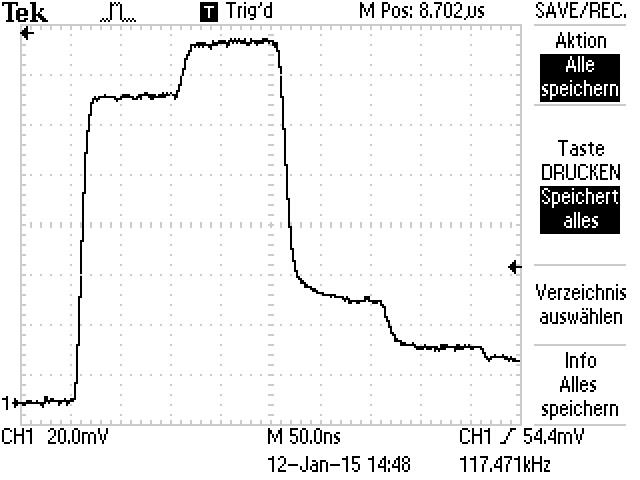
\includegraphics[scale=0.5]{bilder/reflexion/F0001TEK.JPG}
  \caption{Mit dem Oszilloskop aufgenommenes Bild des kurzen \CU-Kabels mit
  kurzgeschlossenem Ende.}
  \label{fig:oszi_50k_kurz}
\end{figure}
\begin{figure}[ht]
  \centering
  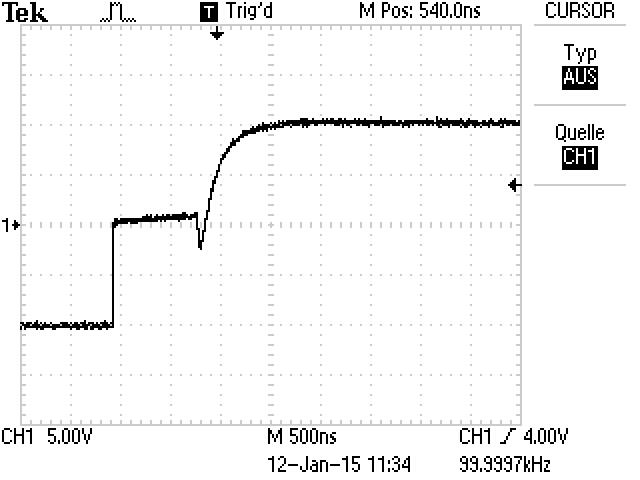
\includegraphics[scale=0.5]{bilder/reflexion/F0002TEK.JPG}
  \caption{Mit dem Oszilloskop aufgenommenes Bild des kurzen \BU-Kabels mit
  offenem Ende.}
  \label{fig:oszi_75k_offen}
  \vspace{2em}
  \includegraphics[scale=0.5]{bilder/reflexion/F0003TEK.JPG}
  \caption{Mit dem Oszilloskop aufgenommenes Bild des kurzen \BU-Kabels mit
  kurzgeschlossenem Ende.}
  \label{fig:oszi_75k_kurz}
\end{figure}
\begin{figure}[ht]
  \centering
  \includegraphics[scale=0.5]{bilder/reflexion/F0004TEK.JPG}
  \caption{Mit dem Oszilloskop aufgenommenes Bild des langen \CU-Kabels mit
  offenem Ende.}
  \label{fig:oszi_50l_offen}
  \vspace{2em}
  \includegraphics[scale=0.5]{bilder/reflexion/F0005TEK.JPG}
  \caption{Mit dem Oszilloskop aufgenommenes Bild des langen \CU-Kabels mit
  kurzgeschlossenem Ende.}
  \label{fig:oszi_50l_kurz}
\end{figure}

% ==================================================
% 	Leitungskonstanten
% ==================================================

\clearpage
\subsubsection{Bestimmung der Leitungskonstanten}
\label{ssub:bestimmung_der_leitungskonstanten}

In diesem und den folgenden Unterkapiteln werden Daten aus den
Abbildungen~\ref{fig:oszi_50l_offen} und~\ref{fig:oszi_50l_kurz} über den
ganzen $t$-Bereich oder nur bestimmte Teilbereiche mit Hilfe des Programms
\texttt{Engauge} digitalisiert, um eine bessere Auswertung der Daten zu
ermöglichen. Des weiteren ist die Bestimmung der Leitungskonstante nur bei
dem langen \CU-Kabel möglich, da nur hier der kapazitive und induktive Verlauf
der Spannung zu sehen ist. Im Folgenden werden daher nun die Leitungskonstanten
des langen \CU-Kabels bestimmt.

\paragraph{Der Widerstandsbelag}
\label{par:der_widerstandsbelag}

Hier wird das Oszillosgraphenbild~\ref{fig:oszi_50l_kurz} digitalisiert.
Die erhaltenen Daten befinden sich in Tabelle~\ref{tab:R_Daten} und werden
in Abbildung~\ref{fig:R_Daten} graphisch dargestellt.
Mit Hilfe der Beziehung
\begin{equation}
  U_1 (1 + \Gamma) = U_0 \quad \Rightarrow \quad \Gamma = \frac{U_0}{U_1} - 1
  \label{eq:Gamma_R}
\end{equation}
kann der Reflektionsfaktor $\Gamma$ bestimmt werden. Einsetzen des Ergebnisses
in
\begin{equation}
  \Gamma = \frac{R-Z_0}{R+Z_0} \quad \Rightarrow \quad
  R = - \frac{Z_0(\Gamma + 1)}{\Gamma - 1}
  \label{eq:R}
\end{equation}
liefert schließlich den gewünschten Widerstandsbelag $R$.
Hierbei gilt für den Wellenwiderstand $Z_0 = \SI{50}{\ohm}$.
Es gilt also $U_0$ und $U_1$ zu bestimmen, wobei $U_0$ die Höhe des Pulses aus
Abbildung~\ref{fig:R_Daten} ist und $U_1$ die Höhe der Spannung nach Abfall des
Pulses. Um die Spannungen $U_1$ und $U_0$ bestimmen zu können, muss zudem eine
Offsetspannung $U_\text{off}$ ermittelt werden.
Die eben genannten Spannungen werden entsprechend
\begin{align}
  \begin{aligned}
    U_\text{off} &= \overline{U(t)}\,, \\
    U_1          &= \overline{U(t)}\,, \\
    U_0          &= \overline{U(t)}\,,
  \end{aligned}
  \qquad
  \begin{aligned}
    &t~< \SI{500}{\nano\second} \\
    \SI{750}{\nano\second}  <~&t~< \SI{1360}{\nano\second} \\
    \SI{2000}{\nano\second} <~&t~< \SI{2250}{\nano\second}
  \end{aligned}
\end{align}
bestimmt, wobei $U(t)$ und $t$ aus Tabelle~\ref{tab:R_Daten} bzw.
Abbildung~\ref{fig:R_Daten} entnommen werden.
Die so berechneten Werte lauten
\begin{align}
  U_\text{off} &= \SI[parse-numbers = false]{14.96 \pm 0.09}{\volt} \\
  U_0 &= \SI[parse-numbers = false]{24.36 \pm 0.09}{\volt} \\
  U_1 &= \SI[parse-numbers = false]{25.79 \pm 0.14}{\volt}~.
\end{align}
Damit berechnet sich der Widerstandsbelag nach Gleichung~\eqref{eq:Gamma_R} und
\eqref{eq:R} zu
\begin{equation}
  \underline{R = $-40.0$           & $19.2$            & $830.0$           & $142.4$           & $1470.0$          & $62.0$           \\
$5.0$             & $18.4$            & $875.0$           & $142.8$           & $1485.0$          & $58.8$           \\
$40.0$            & $18.0$            & $905.0$           & $143.6$           & $1500.0$          & $54.8$           \\
$90.0$            & $17.6$            & $955.0$           & $144.0$           & $1535.0$          & $53.2$           \\
$130.0$           & $19.2$            & $1015.0$          & $144.0$           & $1560.0$          & $50.0$           \\
$170.0$           & $18.8$            & $1055.0$          & $144.0$           & $1595.0$          & $48.0$           \\
$220.0$           & $18.8$            & $1100.0$          & $144.8$           & $1635.0$          & $47.2$           \\
$255.0$           & $18.4$            & $1150.0$          & $144.4$           & $1675.0$          & $45.6$           \\
$295.0$           & $18.4$            & $1195.0$          & $144.8$           & $1720.0$          & $44.4$           \\
$340.0$           & $18.4$            & $1235.0$          & $145.6$           & $1760.0$          & $44.0$           \\
$385.0$           & $18.0$            & $1280.0$          & $145.6$           & $1800.0$          & $43.6$           \\
$425.0$           & $18.8$            & $1330.0$          & $145.6$           & $1850.0$          & $43.2$           \\
$470.0$           & $18.4$            & $1365.0$          & $146.0$           & $1895.0$          & $43.2$           \\
$510.0$           & $19.2$            & $1370.0$          & $142.0$           & $1945.0$          & $43.2$           \\
$515.0$           & $22.8$            & $1375.0$          & $138.4$           & $1980.0$          & $42.8$           \\
$520.0$           & $30.8$            & $1380.0$          & $130.4$           & $2030.0$          & $42.8$           \\
$525.0$           & $38.4$            & $1385.0$          & $118.8$           & $2075.0$          & $43.2$           \\
$530.0$           & $90.4$            & $1390.0$          & $102.8$           & $2120.0$          & $43.2$           \\
$535.0$           & $106.0$           & $1395.0$          & $99.2$            & $2170.0$          & $43.2$           \\
$540.0$           & $122.0$           & $1400.0$          & $95.2$            & $2215.0$          & $43.2$           \\
$550.0$           & $137.6$           & $1405.0$          & $87.6$            & $2260.0$          & $42.8$           \\
$570.0$           & $139.2$           & $1410.0$          & $83.6$            & $2300.0$          & $42.8$           \\
$605.0$           & $140.8$           & $1415.0$          & $80.0$            & $2345.0$          & $42.0$           \\
$645.0$           & $140.4$           & $1420.0$          & $76.0$            & $2390.0$          & $40.8$           \\
$685.0$           & $141.2$           & $1430.0$          & $72.4$            & $2420.0$          & $40.8$           \\
$730.0$           & $141.6$           & $1440.0$          & $68.8$            & -                 & -                \\
$780.0$           & $142.4$           & $1455.0$          & $65.6$            & -                 & -                \\}~.
\end{equation}

% Tabellen und Bilder
\begin{table}[hb]
  \centering
  \begin{tabular}{cc|cc|cc}
    \midrule
    \midrule
    $t / \si{\nano\second}$ & $U / \si{\milli\volt}$ &
    $t / \si{\nano\second}$ & $U / \si{\milli\volt}$ &
    $t / \si{\nano\second}$ & $U / \si{\milli\volt}$ \\
    \midrule
    $-40.0$           & $19.2$            & $830.0$           & $142.4$           & $1470.0$          & $62.0$           \\
$5.0$             & $18.4$            & $875.0$           & $142.8$           & $1485.0$          & $58.8$           \\
$40.0$            & $18.0$            & $905.0$           & $143.6$           & $1500.0$          & $54.8$           \\
$90.0$            & $17.6$            & $955.0$           & $144.0$           & $1535.0$          & $53.2$           \\
$130.0$           & $19.2$            & $1015.0$          & $144.0$           & $1560.0$          & $50.0$           \\
$170.0$           & $18.8$            & $1055.0$          & $144.0$           & $1595.0$          & $48.0$           \\
$220.0$           & $18.8$            & $1100.0$          & $144.8$           & $1635.0$          & $47.2$           \\
$255.0$           & $18.4$            & $1150.0$          & $144.4$           & $1675.0$          & $45.6$           \\
$295.0$           & $18.4$            & $1195.0$          & $144.8$           & $1720.0$          & $44.4$           \\
$340.0$           & $18.4$            & $1235.0$          & $145.6$           & $1760.0$          & $44.0$           \\
$385.0$           & $18.0$            & $1280.0$          & $145.6$           & $1800.0$          & $43.6$           \\
$425.0$           & $18.8$            & $1330.0$          & $145.6$           & $1850.0$          & $43.2$           \\
$470.0$           & $18.4$            & $1365.0$          & $146.0$           & $1895.0$          & $43.2$           \\
$510.0$           & $19.2$            & $1370.0$          & $142.0$           & $1945.0$          & $43.2$           \\
$515.0$           & $22.8$            & $1375.0$          & $138.4$           & $1980.0$          & $42.8$           \\
$520.0$           & $30.8$            & $1380.0$          & $130.4$           & $2030.0$          & $42.8$           \\
$525.0$           & $38.4$            & $1385.0$          & $118.8$           & $2075.0$          & $43.2$           \\
$530.0$           & $90.4$            & $1390.0$          & $102.8$           & $2120.0$          & $43.2$           \\
$535.0$           & $106.0$           & $1395.0$          & $99.2$            & $2170.0$          & $43.2$           \\
$540.0$           & $122.0$           & $1400.0$          & $95.2$            & $2215.0$          & $43.2$           \\
$550.0$           & $137.6$           & $1405.0$          & $87.6$            & $2260.0$          & $42.8$           \\
$570.0$           & $139.2$           & $1410.0$          & $83.6$            & $2300.0$          & $42.8$           \\
$605.0$           & $140.8$           & $1415.0$          & $80.0$            & $2345.0$          & $42.0$           \\
$645.0$           & $140.4$           & $1420.0$          & $76.0$            & $2390.0$          & $40.8$           \\
$685.0$           & $141.2$           & $1430.0$          & $72.4$            & $2420.0$          & $40.8$           \\
$730.0$           & $141.6$           & $1440.0$          & $68.8$            & -                 & -                \\
$780.0$           & $142.4$           & $1455.0$          & $65.6$            & -                 & -                \\
    \midrule
    \midrule
  \end{tabular}
  \caption{Datstellung der digitalisierten Daten des
    Oszillosgraphenbild~\ref{fig:oszi_50l_kurz}.}
  \label{tab:R_Daten}
\end{table}
\begin{figure}[hb]
  \centering
  \includegraphics[scale=1.0]{bilder/R.pdf}
  \caption{Graphische Darstellung der digitalisierten Daten des
    Oszillosgraphenbild~\ref{fig:oszi_50l_kurz}.}
\label{fig:R_Daten}
\end{figure}

\clearpage
\paragraph{Der induktive Belag}
\label{par:der_induktive_belag}

Ein kurzgeschlossenes Koaxialkabel zeigt ein rein induktives Verhalten, daher
wird zur Bestimmung des induktiven Belags ebenfalls das
Oszillosgraphenbild~\ref{fig:oszi_50l_kurz} mit den entsprechend
digitalisierten Daten aus Tabelle~\ref{tab:R_Daten} verwandt.
Jedoch werden diese Daten auf den für den Induktivitätsbelag relevanten Teil
eingeschränkt, sodass nur die Werte $U(t)$ aus
\begin{equation}
  \SI{1430}{\nano\second} <~t~< \SI{2250}{\nano\second}
\end{equation}
betrachtet werden. Diese Werte sind in Abbildung~\ref{fig:induktivitaetsbelag}
graphisch dargestellt.
Die Abfallende Flanke des Pulses entspricht nun einem Ausschaltvorgang
einer Spule entsprechend
\begin{equation}
  U(t) = U_0 \exp(-\frac{t}{\tau}) + U_\text{off} \quad \text{mit} \quad
  \tau = \frac{L}{R+Z_0}~,
  \label{eq:L_abschalt}
\end{equation}
wobei $R$ den oben bestimmten Widerstandsbelag und $U_\text{off}$ die
Offsetspannung zu \SI{0}{\volt} darstellt. Durch Umstellen und Logarithmierung
der Gleichung \eqref{eq:L_abschalt} ergibt sich eine Geradengleichung der Form
\begin{equation}
  \ln(U - U_\text{off}) = -\frac{t}{\tau} + \ln U_0 \coloneqq
  m \cdot t + \ln U_0 \quad \text{mit} \quad m = - \frac{1}{\tau}
\end{equation}
womit schließlich eine lineare Regression durchgeführt und aus der
Steigung der Induktivitätsbelag bestimmt werden kann.
Die Offsetspannung wird entsprechend%
\begin{equation}
  U_\text{off} = \overline{U(t)}\,,
  \quad \SI{2100}{\nano\second} <~t~< \SI{2250}{\nano\second}
\end{equation}
zu%
\begin{equation}
  U_\text{off} = \SI{64.11}{\milli\volt}
\end{equation}
bestimmt.
In Abbildung~\ref{fig:induktivitaetsbelag_fit} sind nun die Daten
${\ln(U - U_\text{off})}$ sowie die dazugehörige lineare Regression eingetragen.
Die entsprechenden Daten befinden sich in Tabelle~\ref{tab:L_Daten}.
Der Fit ergibt dabei die Gleichung
\begin{equation}
  \sisetup{per-mode=reciprocal-positive-first}
  G_L(t) = \SI[parse-numbers = false]{-0.0053 \pm 0.0004}{\per\nano\second}\, \cdot \,t\, + \SI[parse-numbers = false]{11.6 \pm 0.7}{}~.
  \label{eq:L_fit}
\end{equation}
Aus der Steigung von~\ref{eq:L_fit} wird nun mit Gleichung~\eqref{eq:L_abschalt} der
Induktivitätsbelag zu
\begin{equation}
  \underline{L = \SI[parse-numbers = false]{226.0 \pm 4.2}{\milli\henry}}
  \label{eq:indukivitaetsbelag}
\end{equation}
bestimmt.

\begin{table}[htpb]
  \centering
  \begin{tabular}{cccc}
    \midrule
    \midrule
    $t / \si{\nano\second}$ & $U / \si{\milli\volt}$ &
    $U - U_\text{off} / \si{\milli\volt}$ & $\ln(U - U_\text{off})$ \\
    \midrule
    \SI[parse-numbers = false]{226.0 \pm 4.2}{\milli\henry}
    \midrule
    \midrule
  \end{tabular}
  \caption{Darstellung der für den Induktivitätsbelag relevanten Daten sowie
  die berechneten Werte für den Fit.}
  \label{tab:L_Daten}
\end{table}
\begin{figure}[htpb]
  \centering
  \includegraphics[scale=1.0]{bilder/L.pdf}
  \caption{Darstellung der für die zur Bestimmung des Induktivitätsbelags
    relevanten digitalisierten Daten von Abbildung~\ref{fig:oszi_50l_kurz}.}
  \label{fig:induktivitaetsbelag}
  \includegraphics[scale=1.0]{bilder/L_fit.pdf}
  \caption{Darstellung der für die zur Bestimmung des Induktivitätsbelags
    relevanten digitalisierten Daten von Abbildung~\ref{fig:oszi_50l_kurz}.}
  \label{fig:induktivitaetsbelag_fit}
\end{figure}

\clearpage
\paragraph{Der Kapazitätsbelag}
\label{par:der_kapazit_tsbelag}

Entgegen dem Induktivitätsbelag zeigt ein Koaxialkabel mit offenem Ende ein
rein kapazitives Verhalten. Somit wird zur Bestimmung des Kapazitätsbelags das
Oszillosgraphenbild~\ref{fig:oszi_50l_offen} verwandt. Die entsprechenden
digitalisierten Daten sind in Tabelle~\ref{tab:C_roh_Daten} und
Abbildung~\ref{fig:C_roh_Daten} dargestellt.
Die Einschränkung der relevanten Daten bezieht sich hier auf $U(t)$ aus
\begin{equation}
  \quad \SI{1370}{\nano\second} <~t~< \SI{1650}{\nano\second}~.
\end{equation}
Den zu betrachtenden Verlauf entspricht hier einer Aufladekurve eines
Kondensators gemäß
\begin{equation}
  U = U_0\qty(1 - \exp(-\frac{t}{\tau})) \quad \text{mit} \quad
  \tau = RC~,
  \label{eq:Aufladekurve_C}
\end{equation}
wobei $R$ wiederum der obiger Widerstandsbelag ist. Diese Gleichung kann wieder
linearisiert werden zu
\begin{equation}
  \ln(U_0 - U) = - \frac{t}{\tau} + \ln(U_0)~,
\end{equation}
woraus aus der Steigung der Kapazitätsbelag bestimmt werden kann.
Die Sättigungsspannung $U_0$ wird dabei entsprechend
\begin{equation}
  U_0 = \overline{U(t)}\,,
  \quad \SI{2000}{\nano\second} <~t
\end{equation}
zu
\begin{equation}
  U_0 = \SI{311.78}{\milli\volt}
\end{equation}
bestimmt. Die für den Fit relevanten Daten sind in Tabelle~\ref{tab:C_fit}
dargestellt. Der Fit befindet sich in Abbildung~\ref{fig:C_fit}.
Die aus dem Fit erhaltene Gleichung lautet
\begin{equation}
  \sisetup{per-mode=reciprocal-positive-first}
  1375\phantom{.}   & 215.910           & 95.869            & 4.563            \\
1380\phantom{.}   & 225.883           & 85.896            & 4.453            \\
1385\phantom{.}   & 234.859           & 76.920            & 4.343            \\
1390\phantom{.}   & 244.832           & 66.947            & 4.204            \\
1395\phantom{.}   & 253.807           & 57.972            & 4.060            \\
1405\phantom{.}   & 262.781           & 48.998            & 3.892            \\
1420\phantom{.}   & 271.753           & 40.026            & 3.690            \\
1435\phantom{.}   & 279.727           & 32.052            & 3.467            \\
1465\phantom{.}   & 286.697           & 25.082            & 3.222            \\
1490\phantom{.}   & 292.672           & 19.107            & 2.950            \\
1525\phantom{.}   & 296.648           & 15.131            & 2.717            \\
1560\phantom{.}   & 301.622           & 10.157            & 2.318            \\
1600\phantom{.}   & 303.601           & \phantom{0}8.178  & 2.101            \\
1645\phantom{.}   & 305.578           & \phantom{0}6.201  & 1.825            \\~.
  \label{eq:C_fit}
\end{equation}
Aus der Steigung kann nun der Kapazitätsbelag mit Hilfe von
Gleichung~\eqref{eq:Aufladekurve_C} zu
\begin{equation}
  \underline{C = \SI[parse-numbers = false]{1.82 \pm 0.16}{\nano\farad}}
\end{equation}
bestimmt werden.

% Tabellen und Plots
\begin{table}[htpb]
  \centering
  \begin{tabular}{cc|cc|cc}
    \midrule
    \midrule
    $t / \si{\nano\second}$ & $U / \si{\milli\volt}$ &
    $t / \si{\nano\second}$ & $U / \si{\milli\volt}$ &
    $t / \si{\nano\second}$ & $U / \si{\milli\volt}$ \\
    \midrule
    --40\phantom{.}   & \phantom{0}76.824 & \phantom{0}865\phantom{.} & 200.154           & 1560\phantom{.}   & 301.622          \\
\phantom{0}10\phantom{.} & \phantom{0}75.806 & \phantom{0}910\phantom{.} & 201.133           & 1600\phantom{.}   & 303.601          \\
\phantom{0}60\phantom{.} & \phantom{0}76.784 & \phantom{0}955\phantom{.} & 202.113           & 1645\phantom{.}   & 305.578          \\
105\phantom{.}    & \phantom{0}76.766 & \phantom{0}995\phantom{.} & 201.099           & 1690\phantom{.}   & 305.560          \\
150\phantom{.}    & \phantom{0}75.751 & 1030\phantom{.}   & 200.088           & 1735\phantom{.}   & 305.542          \\
190\phantom{.}    & \phantom{0}77.730 & 1070\phantom{.}   & 201.069           & 1775\phantom{.}   & 308.519          \\
235\phantom{.}    & \phantom{0}75.717 & 1115\phantom{.}   & 201.051           & 1815\phantom{.}   & 308.503          \\
285\phantom{.}    & \phantom{0}75.697 & 1160\phantom{.}   & 202.031           & 1860\phantom{.}   & 310.480          \\
330\phantom{.}    & \phantom{0}75.679 & 1210\phantom{.}   & 203.008           & 1910\phantom{.}   & 310.460          \\
375\phantom{.}    & \phantom{0}75.661 & 1255\phantom{.}   & 202.991           & 1955\phantom{.}   & 312.437          \\
415\phantom{.}    & \phantom{0}76.642 & 1295\phantom{.}   & 201.977           & 1995\phantom{.}   & 310.426          \\
455\phantom{.}    & \phantom{0}75.629 & 1340\phantom{.}   & 202.957           & 2030\phantom{.}   & 311.409          \\
500\phantom{.}    & \phantom{0}75.611 & 1365\phantom{.}   & 206.937           & 2070\phantom{.}   & 311.394          \\
515\phantom{.}    & \phantom{0}83.585 & 1375\phantom{.}   & 215.910           & 2120\phantom{.}   & 313.369          \\
520\phantom{.}    & \phantom{0}93.558 & 1380\phantom{.}   & 225.883           & 2160\phantom{.}   & 311.358          \\
525\phantom{.}    & 112.509           & 1385\phantom{.}   & 234.859           & 2200\phantom{.}   & 312.339          \\
530\phantom{.}    & 142.432           & 1390\phantom{.}   & 244.832           & 2240\phantom{.}   & 313.321          \\
535\phantom{.}    & 161.383           & 1395\phantom{.}   & 253.807           & 2280\phantom{.}   & 313.305          \\
540\phantom{.}    & 181.331           & 1405\phantom{.}   & 262.781           & 2325\phantom{.}   & 311.292          \\
565\phantom{.}    & 196.283           & 1420\phantom{.}   & 271.753           & 2370\phantom{.}   & 310.276          \\
600\phantom{.}    & 197.267           & 1435\phantom{.}   & 279.727           & 2405\phantom{.}   & 311.260          \\
640\phantom{.}    & 196.253           & 1465\phantom{.}   & 286.697           & 2450\phantom{.}   & 310.244          \\
680\phantom{.}    & 199.230           & 1490\phantom{.}   & 292.672           & -                 & -                \\
720\phantom{.}    & 199.214           & 1525\phantom{.}   & 296.648           & -                 & -                \\
    \midrule
    \midrule
  \end{tabular}
  \caption{Darstellung der digitalisierten Daten aus dem
    Oszillosgraphenbild~\ref{fig:oszi_50l_offen}.}
\label{tab:C_roh_Daten}
\end{table}

\begin{table}[htpb]
  \centering
  \begin{tabular}{cccc}
    \midrule
    \midrule
    $t / \si{\nano\second}$ & $U / \si{\milli\volt}$ &
    $U_0 - U / \si{\milli\volt}$ & $\ln(U_0 - U) / \si{\milli\volt}$ \\
    \midrule
    1375\phantom{.}   & 215.910           & 95.869            & 4.563            \\
1380\phantom{.}   & 225.883           & 85.896            & 4.453            \\
1385\phantom{.}   & 234.859           & 76.920            & 4.343            \\
1390\phantom{.}   & 244.832           & 66.947            & 4.204            \\
1395\phantom{.}   & 253.807           & 57.972            & 4.060            \\
1405\phantom{.}   & 262.781           & 48.998            & 3.892            \\
1420\phantom{.}   & 271.753           & 40.026            & 3.690            \\
1435\phantom{.}   & 279.727           & 32.052            & 3.467            \\
1465\phantom{.}   & 286.697           & 25.082            & 3.222            \\
1490\phantom{.}   & 292.672           & 19.107            & 2.950            \\
1525\phantom{.}   & 296.648           & 15.131            & 2.717            \\
1560\phantom{.}   & 301.622           & 10.157            & 2.318            \\
1600\phantom{.}   & 303.601           & \phantom{0}8.178  & 2.101            \\
1645\phantom{.}   & 305.578           & \phantom{0}6.201  & 1.825            \\
    \midrule
    \midrule
  \end{tabular}
  \caption{Darstellung der für den Fit relevanten Daten.}
\label{tab:C_fit}
\end{table}

\begin{figure}[htpb]
  \centering
  \includegraphics[scale=1.0]{bilder/C.pdf}
  \caption{Graphische Darstellung der digitalisierten Daten des langen
    \CU-Kabels mit offenem Ende.}
\label{fig:C_roh_Daten}
  \includegraphics[scale=1.0]{bilder/C_fit.pdf}
  \caption{Graphische Darstellung der digitalisierten Daten des langen
    \CU-Kabels mit offenem Ende.}
\label{fig:C_fit}
\end{figure}

% ==================================================
% 	Schmitt-Diagramm
% ==================================================

\clearpage
\subsubsection{Bestimmung der Kabellänge über ein Smith-Diagramm}
\label{ssub:bestimmung_der_kabell_nge_ber_ein_smith_diagramm}

Nun soll die Länge des langen \BU-Kabels (die Leitungskonstanten der anderen
Kabel konnten wie oben beschrieben nicht bestimmt werden) mit Hilfe eines
Smith-Diagramms bestimmt werden. Die vollständige Umdrehung der
Smith-Diagramms entspricht einer halben Wellenlänge $\lambda$, sodass die
Länge des Kabels durch
\begin{equation}
  l = \frac{\lambda}{2} \cdot \frac{\varphi}{2 \pi}
\end{equation}
angegeben werden kann, wobei $\varphi$ die Phasenverschiebung nach der Reflexion
am Kabelende beschreibt. Die Wellenlänge lässt sich zudem durch
\begin{equation}
  \lambda = \frac{c}{f \sqrt{\epsilon_r}}
\end{equation}
ausdrücken.
Das heißt, gesucht ist zunächst die Phasenverschiebung $\varphi$.
Dazu wird nun der kurzgeschlossene Fall betrachtet.
Die Impedanz des Kabels beträgt hier
\begin{equation}
  Z_L = R + \text{i}\, 2 \pi f L~,
\end{equation}
wobei $R$ und $L$ die oben bestimmten Widerstands- bzw. Induktivitätsbeläge
sind. Somit ergibt sich die Impedanz zu
\begin{equation}
  Z_L = \SI{(8.71 + 0.06i)}{\ohm}~.
\end{equation}
Die Phasenverschiebung $\varphi$ kann nun beschrieben werden als Winkel
zwischen den Reflexionsfaktoren
\begin{equation}
  \Gamma_{L,R} = \frac{Z - Z_0}{Z + Z_0}\,, \quad Z = R, Z_L~,
  % -0.70 + 0.00i
\end{equation}
wobei
\begin{equation}
  \Gamma_R = \SI[parse-numbers = false]{-0.7009 \pm 0.0025}{}~,
\end{equation}
der Reflektionsfaktor am Ende des Kabels,
aus Gleichung \eqref{eq:Gamma_R} gegeben ist.
Damit kann nun die Phase mit
\begin{equation}
  \varphi = \measuredangle(\Gamma_L, \Gamma_R)
\end{equation}
berechnet werden, womit sich schließlich für die Länge
\begin{equation}
  l_L = \underline{\SI{32.0}{\meter}}
\end{equation}
ergibt.
Im offenen Fall gilt
\begin{align}
  \Gamma_R &= 1 \\
  Z_L &= - \frac{i}{2\pi\ fC}~.
\end{align}
Hiermit wird die analog zum kurzgeschlossenen Fall die Länge zu
\begin{equation}
  L_C = \SI{19.8}{\meter}
\end{equation}
bestimmt.

% ==================================================
% 	Mehrfachreflexion
% ==================================================

\subsection{Mehrfachreflexion}
\label{sub:mehrfachreflexion}

In diesem Teil sollen Reflexionen betrachtet werden, die entstehen, wenn zwei
Kabel mit unterschiedlichem Widerstand hintereinandergeschaltet werden.
In diesem Fall das kurze \CU und das kurze \BU-Kabel.
Das aufgenommene Oszillosgraphenbild und die entsprechend digitalisierten Werte
sind in Abbildung~\ref{fig:mehrfachreflexion_roh}
bzw.~\ref{fig:mehrfachreflexion} dargestellt.
Nun werden wieder die Werte der Spannungsplateaus gemittelt, um die
Spannungsflanken und schließlich die Reflexionsfaktoren zu bestimmen.
Die hier verwandten Werte ergeben sich aus
\begin{align*}
  \begin{aligned}
    U_\text{off} &= \overline{U(t)}\,, \\
    U_0          &= \overline{U(t)}\,, \\
    U_1          &= \overline{U(t)}\,, \\
    U_2          &= \overline{U(t)}\,, \\
    U_3          &= \overline{U(t)}\,,
  \end{aligned}
  \qquad
  \begin{aligned}
    &t~< \SI{80}{\nano\second} \\
    \SI{110}{\nano\second} <~&t~< \SI{180}{\nano\second} \\
    \SI{210}{\nano\second}  <~&t~< \SI{285}{\nano\second} \\
    \SI{322}{\nano\second} <~&t~< \SI{380}{\nano\second} \\
    \SI{432}{\nano\second} <~&t
  \end{aligned}
\end{align*}
mit den Ergebnissen
\begin{align*}
  U_\text{off} &= \SI[parse-numbers = false]{202.0 \pm 0.8}{\milli\volt} \\
  U_0 &= \SI[parse-numbers = false]{202.0 \pm 0.8}{\milli\volt} \\
  U_1 &= \SI[parse-numbers = false]{224.5 \pm 1.0}{\milli\volt} \\
  U_2 &= \SI[parse-numbers = false]{330.4 \pm 1.7}{\milli\volt} \\
  U_3 &= \SI[parse-numbers = false]{330.4 \pm 1.7}{\milli\volt}~.
\end{align*}
Von diesen Spannungen wird die Offset-Spannung abgezogen und die folgenden
Spannungsdifferenzen berechnet.
\begin{align*}
  \Delta U_1 &= U_1 - U_0 \\
  \Delta U_2 &= U_2 - U_1 \\
  \Delta U_3 &= U_3 - U_2~.
\end{align*}
Hiermit lassen sich nun die Reflexionsfaktoren zu
\begin{align*}
  \Gamma_L &= \frac{\Delta U_1}{U_0} = \SI[parse-numbers = false]{0.183 \pm 0.012}{} \\
  \Gamma_E &= \frac{\Delta U_3}{\Delta U_2} +
  \frac{\Delta U_2}{U_0(1 - \Gamma_L)}
  = \SI[parse-numbers = false]{0.916 \pm 0.023}{} \\
  \Gamma_R &= \frac{\Delta U_3}{\Delta U_2 \Gamma_E}
  = \SI[parse-numbers = false]{-0.152 \pm 0.019}{}
\end{align*}
bestimmen.
Die Reflexionsfaktoren $\Gamma_L$ und $\Gamma_R$ sollten nach der Theorie
betragsmäßig ca. 0.2 sein. Somit ist anzunehmen, dass die verwandten Kabel von
ihrer Nennimpedanz abweichen.

\begin{figure}[htpb]
  \centering
  \includegraphics[scale=0.6]{bilder/mehrfachreflexion/F0000TEK.JPG}
  \caption{Aufgenommenes Oszillosgraphenbild bei hintereinandergeschalteten
    \CU- und \BU-Kabel.}
\label{fig:mehrfachreflexion_roh}
  \includegraphics[scale=1.0]{bilder/mehrfachreflexion/mf.pdf}
  \caption{Darstellung der digitalisierten Daten aus dem
    Oszilloskopenbild aus Abbildung~\ref{fig:mehrfachreflexion_roh}}
\label{fig:mehrfachreflexion}
\end{figure}

\subsection{Spannungsverlauf bei drei verschiedenen Abschlusswiderständen}
\label{sub:spannungsverlauf_bei_drei_verschiedenen_abschlusswiderst_nden}

In diesem Versuchsteil sollen die Spannungsverläufe mit drei unterschiedlichen,
noch unbekannten, Abschlusswiderständen untersucht werden.
Hierbei wird das kurze \CU-Kabel verwandt.

\paragraph{Abschluss 3}
\label{ssub:abschluss_3}

Der Spannungsverlauf ist in Abbildung~\ref{fig:abschluss_3} dargestellt.
Im Vergleich der im Anhang befindlichen Abbildung~\ref{fig:abschluesse} handelt
es sich hier um Abschluss, welcher aus einer Parallelschaltung von einem
Widerstand mit einem Kondensator besteht.

\paragraph{Abschluss 4}
\label{ssub:abschluss_4}

Der Spannungsverlauf des Signals mit Abschluss 4 ist in
Abbildung~\ref{fig:abschluss_4} dargestellt. Hierbei handelt es sich um eine
Reihenschaltung von einem Widerstand mit einer Spule.

\paragraph{Abschluss 1}
\label{par:abschluss_1}

Hier befindet sich der Spannungsverlauf in Abbildung~\ref{fig:abschluss_1}.
Der Vergleich mit den Abschlüssen in Abbildung~\ref{fig:abschluesse} liefert
hier einen Abschlusswiderstand, welcher aus einer Reihenschaltung eines
Widerstandes und einem Kondensator besteht.


\begin{figure}[htpb]
  \centering
  \fbox{\includegraphics[scale=0.45]{bilder/abschluss/F0003TEK.JPG}}
  \caption{Spannungsverlauf mit Abschlusswiderstand 3.}
\label{fig:abschluss_3}
\end{figure}

\begin{figure}[htpb]
  \centering
  \fbox{\includegraphics[scale=0.5]{bilder/abschluss/F0004TEK.JPG}}
  \caption{Spannungsverlauf mit Abschlusswiderstand 4.}
\label{fig:abschluss_4}
  \vspace{2em}
  \fbox{\includegraphics[scale=0.5]{bilder/abschluss/F0005TEK.JPG}}
  \caption{Spannungsverlauf mit Abschlusswiderstand 1.}
\label{fig:abschluss_1}
\end{figure}


%
% ==================================================
%	Diskussion
% ==================================================
\clearpage
\section{Diskussion}
In Tabelle \ref{tab:ergebnisse} sind noch einmal die Ergebnisse 
dieser Versuchsdurchführung und die entsprechenden Literaturwerte 
aufgelistet.

\begin{table}[h]
\centering
\begin{tabular}{crc}
\toprule \midrule
Physikalische Größe & Ermittelter Wert & Literaturwert \\
\midrule
$k_\text{B}$ 	& 41.8+/-0.8
$\times 10^{-23}\frac{\text{J}}{\text{K}}$ & $1.380 648 
52(79)\times 10^{-23}\frac{\text{J}}{\text{K}}$\cite{pdg}		\\
"  				& 0.171+/-0.005
$\times 10^{-23}\frac{\text{J}}{\text{K}}$ & "		\\ 
"  				& 1.3+/-0.4
$\times 10^{-23}\frac{\text{J}}{\text{K}}$ & "		\\
"  				& 9.6+/-3.2
$\times 10^{-23}\frac{\text{J}}{\text{K}}$ & "		\\
$\text{e}_0$		& (6.39+/-0.14)e-25
$\times 10^{-19}\text{C}$ & $1.602 176 6208(98)\times 
10^{-19}$C\cite{pdg} \\
$\alpha$			& 0.66+/-0.24 
&$\mathcal{O}(1)$\\
\midrule
\bottomrule
\end{tabular}
\caption{Zusammenstellung der Versuchsergebnisse.}
\label{tab:ergebnisse}
\end{table}


%cite{pdg} http://pdg.lbl.gov/2015/reviews/rpp2015-rev-phys-constants.pdf


Bei den ermittelten Werten für die Boltzmankonstante $k_\text{B}$ 
zeigen sich für die Messungen am einfachen Rauschspektrometer 
(erste zwei Werte) eine deutlich größere Abweichung vom Literaturwert 
im vergleich zu den Messungen am Rauschspektrometer nach 
Korrelationsprinzip. Aus den in der Theorie genannten Gründen 
war dieses Verhalten bereits zu erwarten. Insbesondere der Wert 
$k_\text{B}=1.3+/-0.4$ am korrelierten Spektrometer 
mit kleinem Widerstand $R$ bis $1000\Omega$ enthält den Literaturwert 
in seinem Toleranzbereich. 

Der ermittelte Wert für die Elementarladung $\text{e}_0$ weicht 
geringfügig nach unten ab. Eine mögliche Begründung für diese 
Verschiebung ist, dass während der Messreihe die Kathode wieder 
an eine externe Stromquelle angeschlossen war und nicht allein 
vom Bleiakkumulator betrieben wurde, sodass Störsignale den 
Rauscheffekt beeinflusst haben könnten.

Der Exponent des Funkeleffekts, der als Repräsentant eines $1/f$ 
Rauschens untersucht wurde, liegt wie erwartet in der Größenordnung 
von $1$, sodass hier wirklich von einem $1/\nu^\alpha\approx 1/\nu$ 
Rauschen gesprochen werden kann. Wie ebenfalls erwartet trat der 
Funkeleffekt bei der Oxydkathode deutlich stärker auf als bei 
der Reinmetallkathode (vgl. dazu Abb. \ref{fig:kathode_rein} und 
\ref{fig:kathode_oxyd})  .

% ==================================================
%	Literaturverzeichnis
% ==================================================

% \referenzen

% ==================================================
%	Dokument endet
% ==================================================

\end{document}
